%%%%%%%%%%%%%%%%%%%%%%%%%%%%%%%%%%%%%%%%%%%%%%%%%%%%%%%%%%%%%%%%%%%%%%%%%%%%%%%%
%2345678901234567890123456789012345678901234567890123456789012345678901234567890
%        1         2         3         4         5         6         7         8

\documentclass[letterpaper, 10 pt, conference]{ieeeconf} 
%\usepackage{times}
\usepackage{algorithmic}
\usepackage{algorithm}
\usepackage{subcaption}
%\documentclass[a4paper, 10pt, conference]{ieeeconf}      % Use this line for a4 paper

% See the \addtolength command later in the file to balance the column lengths
% on the last page of the document

% The following packages can be found on http:\\www.ctan.org
%\usepackage{graphics} % for pdf, bitmapped graphics files
%\usepackage{epsfig} % for postscript graphics files
%\usepackage{mathptmx} % assumes new font selection scheme installed
%\usepackage{times} % assumes new font selection scheme installed
%\usepackage{amsmath} % asRRTLearnICRAsumes amsmath package installed
%\usepackage{amssymb}  % assumes amsmath package installed
\usepackage{mathtools}
\usepackage{amsmath}
%\usepackage{amsfonts}
\usepackage{color}
\usepackage{amssymb}
\DeclareMathOperator*{\argmin}{\arg\!\min} 
\DeclareMathOperator*{\argmax}{\arg\!\max} 

% \title{\LARGE \bf
% Rapidly Exploring Learning Trees
% }
\IEEEoverridecommandlockouts                              % This command is only needed if 
                                                          % you want to use the \thanks command

\overrideIEEEmargins  

\title{\LARGE \bf
Learning social interaction behaviours for robotic Telepresence via demonstrations and Deep Learning
}


\author{Kyriacos Shiarlis$^{1}$, Joao Messias$^{1}$, and Shimon Whiteson$^{2}$% <-this % stops a space
% \thanks{*This work was not supported by any organization}% <-this % stops a space
\thanks{$^{1}$Informatics Institute, University of Amsterdam, The Netherlands,
         {\tt\small \{k.c.shiarlis,j.messias\}@uva.nl}}%
\thanks{$^{2}$Department of Computer Science, University of Oxford, United Kingdom,
         {\tt\small shimon.whiteson@cs.ox.ac.uk}}%
}



% \author{Kyriacos Shiarlis \\
% University of Amsterdam \\
% k.c.shiarlis@uva.nl
% \And 
% Joao Messias \\
% University of Amsterdam \\ 
% jmessias@uva.nl 
% \And
% Shimon Whiteson \\
% University of Oxford \\
% shimon.whiteson@cs.ox.ac.uk 
% }
\newcommand{\jm}[1]{\textcolor{blue}{Joao: #1}}

\newcommand{\sw}[1]{\textcolor{red}{SW: #1}}
\newcommand{\ks}[1]{\textcolor{green}{KS: #1}}


\begin{document}

\maketitle

\thispagestyle{empty}
\pagestyle{empty}


%%%%%%%%%%%%%%%%%%%%%%%%%%%%%%%%%%%%%%%%%%%%%%%%%%%%%%%%%%%%%%%%%%%%%%%%%%%%%%%%
\begin{abstract}
The increasing amount of robots in public and social spaces increases the need for robots to be able to perform even the simplest tasks in a socially appropriate manner. However, coding social behaviours into robots can be a daunting task, as a lot of manual tuning might be required in order to achieve the required result. More importantly, coding such behaviours is technically inaccessible to non-experts.  In such cases Learning from Demonstration (LfD) \cite{argall2009survey} can be a powerful tool for robotisists. In this work we describe a generic neural network architecture and use it to learn two social robotic tasks for a telepresence robot. We carefully reason about the choice of the architecture and show that all aspects are important using ablation experiments.  We further demonstrate that our method performs better than a naïve controller and a Gradient Boosting Regression method, therefore demonstrating that all elements of our architecture are essential to success. 

\end{abstract}


%%%%%%%%%%%%%%%%%%%%%%%%%%%%%%%%%%%%%%%%%%%%%%%%%%%%%%%%%%%%%%%%%%%%%%%%%%%%%%%%
\section{Introduction}


In recent years robots have been finding their way out of conventional constrained industrial environments and into more social and less structured ones such as museums \cite{thrun1999minerva}, airports \cite{triebel2015spencer}, restaurants \cite{qing2010research} and care centers \cite{shiarlis2015teresa}. This shift poses countless challenges for many aspects of robotics from hardware all the way to high level behaviour design.  One challenge that arises in social environments is that of personalisation. For example the social distance and pose that a robot should maintain when facing a group of people might vary from place to place \cite{joosse2014cultural}. This means that the robot's designer's should design the robot such that parameters can be changed. Additionally, social behaviors might be hard to program manually, for example how a robot should approach a group of people is still the subject of ongoing research \cite{vroon2015dynamics}. Finally, it would be favourable if non-roboticists could program different robot behaviours as they please without a technical expert. For these challenges Learning from Demonstration(LfD) is a powerful tool. Instead of programming behaviours manually LfD, employes human demonstrations along with learning algorithms, whose aim is to extract the program from the data. This means that complex social behaviours that would require carefuly crafted programs can be learned from demonstrations. More importantly, if the learning algorithms are sufficiently generic, these demonstrations no longer need to be coming from a roboticist, but from anyone that is capable on controlling the robot. 

To achieve this however, LfD would need to surpass a few challenges of its own. Firstly as mentioned above, the learning algorithms need to be sufficiently generic. If for example we are learning low level behaviors for a mobile robot, we should be able to learn a wide set of behavious with a single learning algorithm, only by varying the data. Failure to do so would mean that each behaviour would require us to program a different learning procedure which would take away much of the benefit of LfD. 

Another challenge that is especially relevant in social robotics is the robustness of the robot's perception, due to the highly unstructured nature of the environment and limitations in the sensors. Noisy perception can greatly confuse LfD methods if those are not designed to be robust it. As an example consider a social robot that is supposed to follow a person in a relatively crowded space. The robot must maintain the belief about the identity of the person it is following, furthermore it should be robust to false positive people detections within the environment. Failure to do so would result in the robot 'misunderstaning' what the demonstrations wanted to show.

 Recent advancements in Deep Learning allow computers and robots to perform many learning tasks with a single neural network architecture [atari]. In addition certain methods within the field have shown robustness to noisy time-dependent inputs allowing the machine to learn many aspects of the environment that previous methods would assume a hand coded model for. For example the system might learn to ignore sensor readings or detections with certain characteristics if that is found to degrade the performance of the system. In this paper we employ a Deep Learning architecture to learn two simple low level behaviors for a holonomic telepresence Robot from demonstration. The first behaviour has to do with reconfiguration of the robot when interacting with a group. Taking that is, the correct body pose in the presence of a group of people of changing size and position. The second behaviour is following two people in abitrary formation. The rest of the paper is organised as follows. Section 2 describes the behaviours we wish to learn, summarises related work in the field and describes the experiments performed to collect the required data. Section 3 explains the challenges inherent in the tasks and the collected data. Through these challenges we explain the design choices for our neural network architecture. Section 4 describes quantitative and qualitative evaluation of our system against baselines. We remove different aspects of our architecture to show that all aspects are important. Furthermore we benchmark our method against a Gradient Boosting Regression baseline. Section 5 concludes the paper and details our plans for further work.

% In path planning, Rapidly Exploring Random Trees (RRTs)~\cite{lavalle1998rapidly} are popular because they cope well with continuous and high-dimensional domains. The RRT$^*$ algorithm , which extends RRTs to incorporate a cost function, is especially effective. However, the cost functions used by RRT$^*$ are typically simple and hand-coded and, to our knowledge, no methods have been developed to learn RRT$^*$ cost functions from demonstrations.


% In this paper, we propose Rapidly Exploring Learning Trees (), which learns RRT$^*$ cost functions from demonstration. Specifically we modify Maximum Margin Planning to use RRT$^*$ as a planner.  RLT$^*$ requires no additional planner assumptions other than those inherent in RRT$^*$, making it particularly easy to implement. 

\section{Problem Statement \label{sec:related_work}}


In this paper we will use LfD to learn social interaction behaviors for telepresence robots \cite{kristoffersson2013review}, i.e. robots that act as avatars for a remotely present \emph{pilot} which is in charge of the machine's control. The pilot is telepresent and in conversation with one or more \emph{interaction target(s)}. We aim to learn behaviors (tasks\footnote{Note that in this paper we will use behavior and task interchangably. E.g. a \emph{follow} task and behavior both refer to the robot following one or more people.}) that aim to automate the low level control of this robot so that the pilot would only give high level commands, e.g, \emph{converse} or \emph{follow}. Note however that the tasks described in this section are general enough and thus their application is not confined to telepresence. In solving this problem we firstly assume that the robot is equiped with means of detecting people around it. Secondly we assume that the robot operates "in the wild" and not in a "laboratory" setting. This means that there could be a people in the room that are not involved in the conversation as well as sources of false positive people detections. In the rest of this section we describe the behaviors we want to learn as well as the data collected in order to achieve this task. 

\subsection{Behaviors \label{subsec:behaviors}}

\paragraph{Group Reconfiguration Behaviour} In this task the robot is conversing with one or more interaction target(s). At some point the configuration of the group changes, for example someone joins or leaves the group, the group changes shape or simply moves. The robot should reconfigure itself appropriately so as to facilitate conversation in the new situation. Furthermore the robot should remain indifferent to people that are detected but clearly not part of the conversation group. The task is shown diagrammatically in Figure \ref{fig:static}. This task is challenging because it can be hard to hard code what a group of people looks like and then design a general enough behavior for all cases that might arise.

The task of repositioning a robot following a change in a conversation group's size and shape has been tackled previously by \cite{kuzuoka2010reconfiguring} and \cite{vroon2015dynamics}. In both pieces of work what is investigated are the effects that a robot's behaviour has on people. In our case we automate such a behaviour using LfD methods.  There is furthermore some work on detecting groups of people in crowded environments \cite{lau2010multi} and then building systems that interact with them. In our work the notion of a group is never explicitly defined. Since we are learning a mapping from detections to output actions. This means reduced the amount of programming required for "intermediate" modules, but could potentially increase the amount of data needed for learning.

Knox et al \cite{knox2013training} train a robot to perform tasks that are similar to our group re-alignment task, such as maintaining a conversational distance and "magnetic control". However training is done using human generated reward and reinforcement learning through the TAMER framework \cite{knox2009interactively}. Furthermore, the tasks only consider a single person in the scene and perfect sensing, our work contains no such assumptions.

	\begin{figure}[tbh]
%	\hspace{-5cm}
	\centering
      \begin{subfigure}[b]{0.39\columnwidth}
    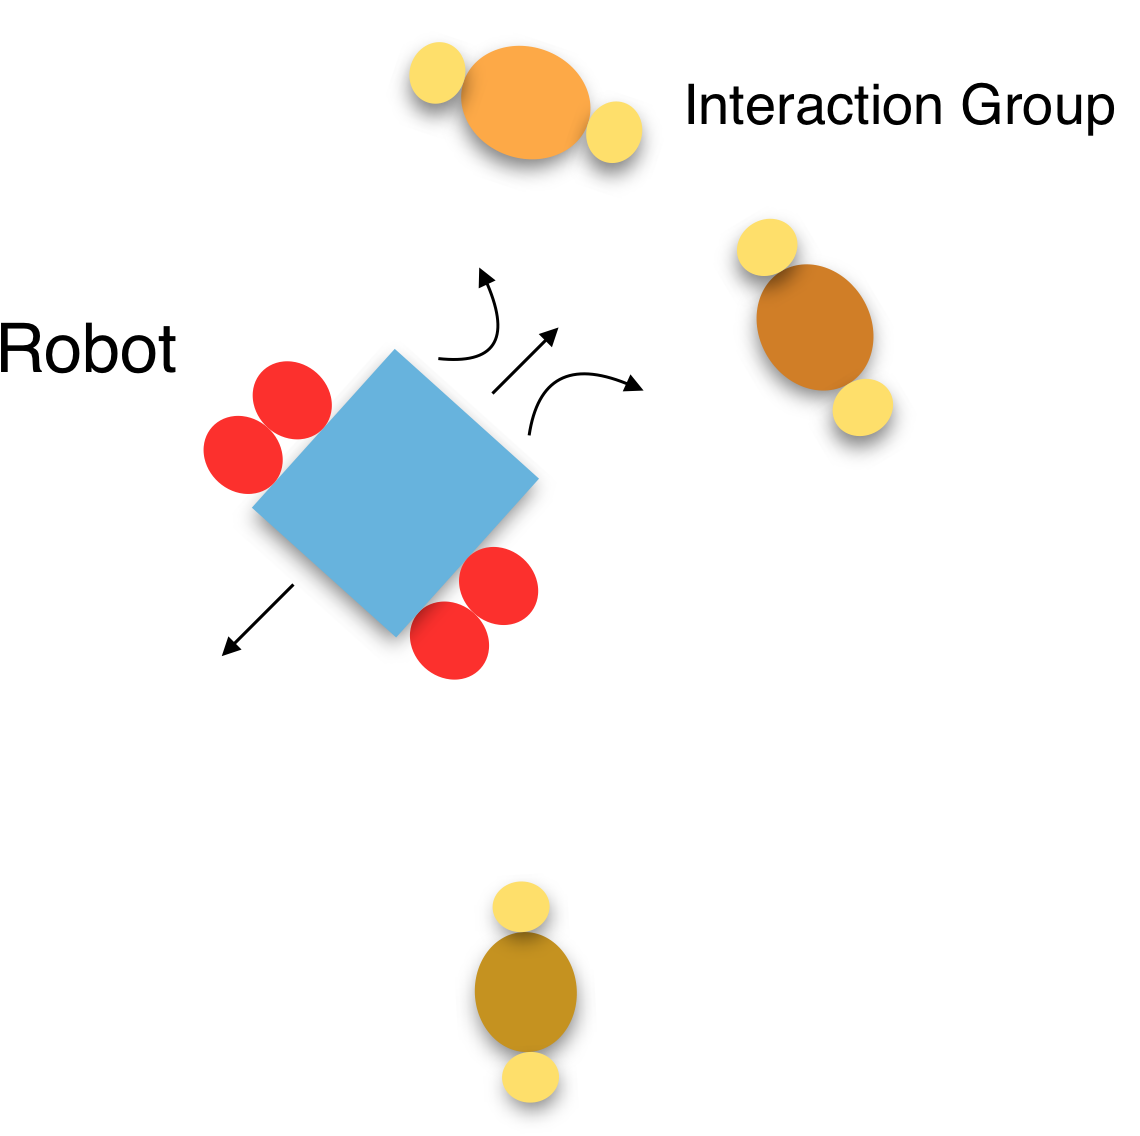
\includegraphics[scale = 0.15]{images/static.png}
    \caption{Group reconfiguration}
    \label{fig:static}
  \end{subfigure}
  \hspace{10mm}
  \begin{subfigure}[b]{0.39\columnwidth}
  \hspace{4mm}
    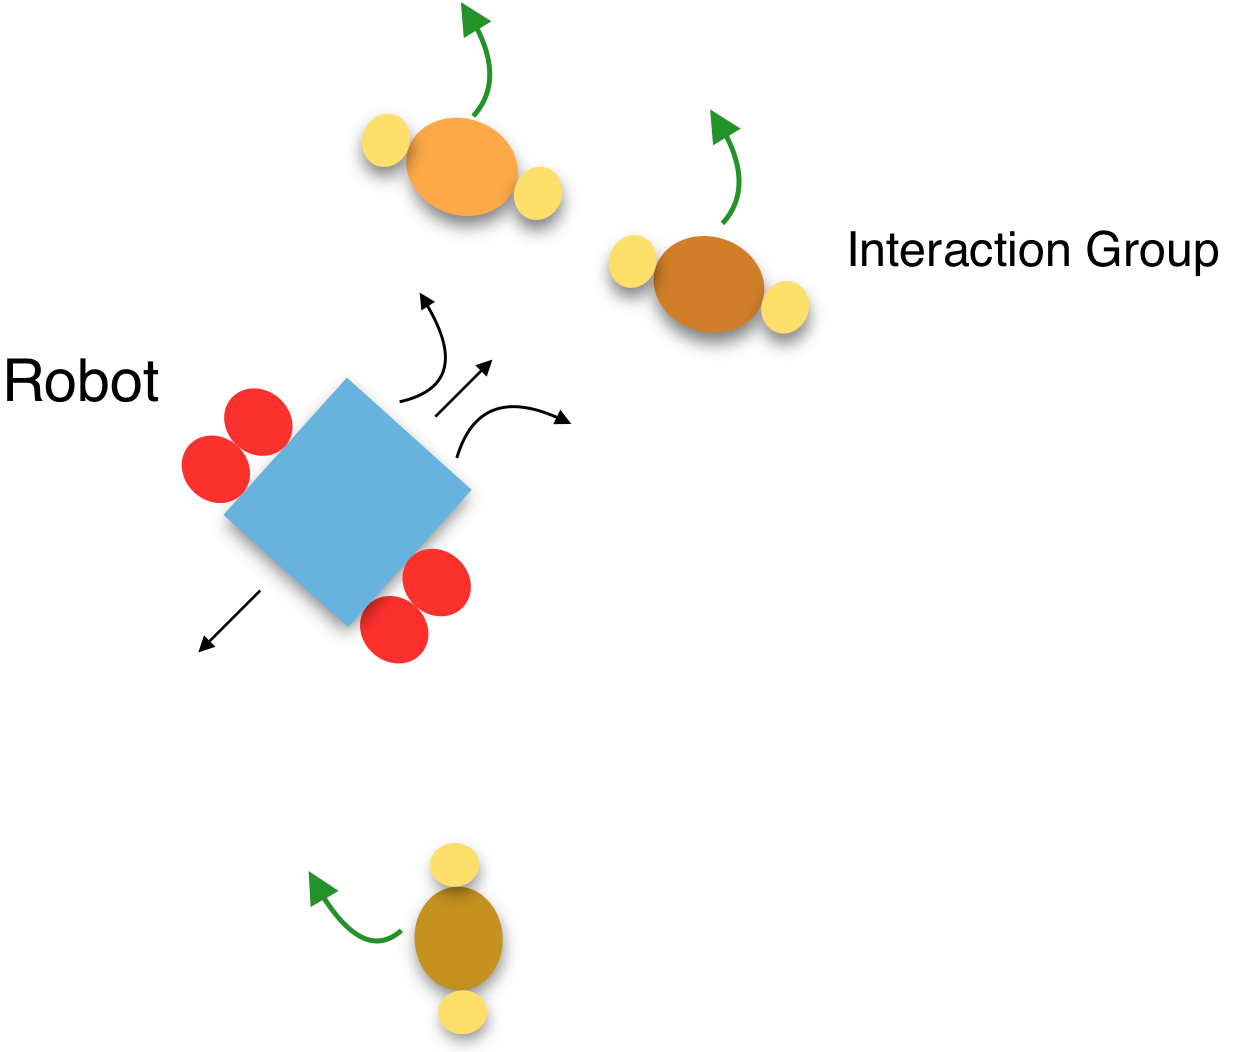
\includegraphics[scale = 0.15]{images/follow.png}
    \caption{Follow}
    \label{fig:follow}
  \end{subfigure} 
  %\vspace{-3mm}
  \caption{(a) The group reconfiguration behavior. Arrows show possible decisions by the robot.  (b) Follow behavior. Arrows show the motion of the robot and the people in the scene.}

    \vspace{-2mm}

  %\vspace{-3mm}
  \label{fig:behaviors}
  \end{figure}

\paragraph{Following bahavior} Here the interaction target(s) are moving and the robot should follow them. The robot should be able to deal with relative variability in the formation of the people it is following. Furthermore it should be robust to false positive detections and be able to retain a following behaviour despite other people that are detected during the task but not relevant to it. This task is shown diagrammatically in Figure \ref{fig:follow}. Following behaviors can be challenging as the sensors might suffer from reliability issues as velocities increase \cite{kobilarov2006people}.

Our second task of having the robot robustly follow people has also been popular among robotisists. A recent method described in \cite{ferrer2016robot} uses an extended social force model enriched with a goal prediction module in order to allow to walk side by side with a person. Furthermore, the system tests different social forces parameters and allows the user to give feedback about the experience. Based on this feedback the robot learns to adapt itself to the specific person.  Our work investigates the possibility of bypassing such models and simply learn the required behavior robustly through data.  

It is interesting to note that none of the work above employs Learning from Demonstration to learn how a robot should behave socially. LfD seems to be instead most commonly used for complex manipulation tasks \cite{argall2009survey} where the field is indeed very active. In terms of social robot behavior LfD is mostly used for learning high level behaviours . Our work fills this gap, by learning low level control of a social robot  from demonstrations.

Another crucial issue that we would like to address is that in many cases, even though the environment around the robot changes, there should be no change in the behavior of the robot. This \emph{invariance} is very hard to hard code. For example if we were to use a social force model to solve the tasks, the calculated forces would vary all the time based on the people position. This in turn means that the behavior of the robot could become either over or under sensitive depending on tuning. By learning these behaviors from demonstrations we hope that the robot will not only learn what to do and how to do it, but also when to do it.


\subsection{Data and Experiments \label{subsec:data_exp}} 

To collect that data required for learning we have performed one set of experiments for each of the tasks described above. Every experimental session consisted of two experimenters, one or more volunteers from the University of Amsterdam and a TERESA\footnote{www.teresaproject.eu} intelligent telepresence system, shown in Figure \ref{fig:robot}.  One experimenter would act as the pilot while the other would be on the other side of the interaction and would have two roles. The first role would be to act as an interaction target. The second would be to instruct the volunteers to join or leave the interaction and attempt to change the shape of the interaction group (triggering an appropriate reaction from the pilot) in order to capture sufficient variability in the data.  

During these interactions, we record the positions of all people detected and tracked by the robot. We also record a binary label, indicating the primary interaction target for the robot. The primary interaction target is defined as the most important person in the interaction and it is defined by the pilot. The observation $o_t$ of $K$ people tracked at time $t$ where the first person is the primary interaction target is therefore defined as, $o_t = \{(\rho_1,\phi_1,1), (\rho_2,\phi_2,0),(\rho_3,\phi_3,0) ... (\rho_{K_t},\phi_{K_t},0)\}_t$, where $\rho_k$ is the distance from the robot and $\phi_k$ is the angle from the robot. This is shown in Figure \ref{fig:data}. We in addition recorded the linear and angular velocity commands given by the pilot, $a_t = (v_t,\omega_t)$, where $a_t$ denotes the action at time $t$. Recording took place at 10Hz, which amounts to the control rate we would use for the robot.  It is also worth noting that these interactions took place in different environments each containing different amounts of people and different sources of false possitives for the people detection modules.

  	\begin{figure}[tbh]
	\centering
      \begin{subfigure}[b]{0.35\columnwidth}
    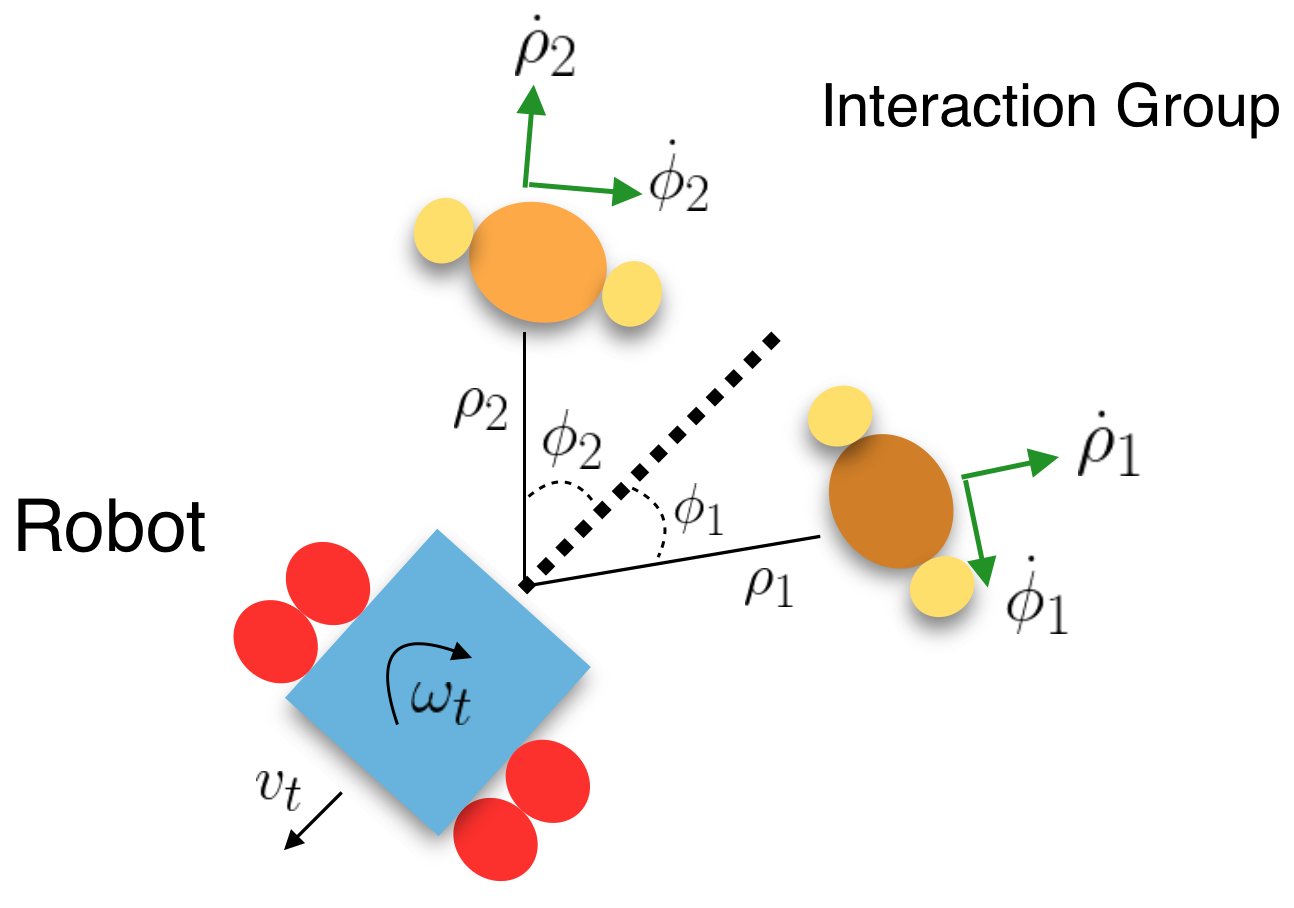
\includegraphics[scale = 0.19]{images/data.png}
    \caption{}
    \label{fig:data}
  \end{subfigure}
  \hspace{10mm}
  \begin{subfigure}[b]{0.35\columnwidth}
  \hspace{4mm}
    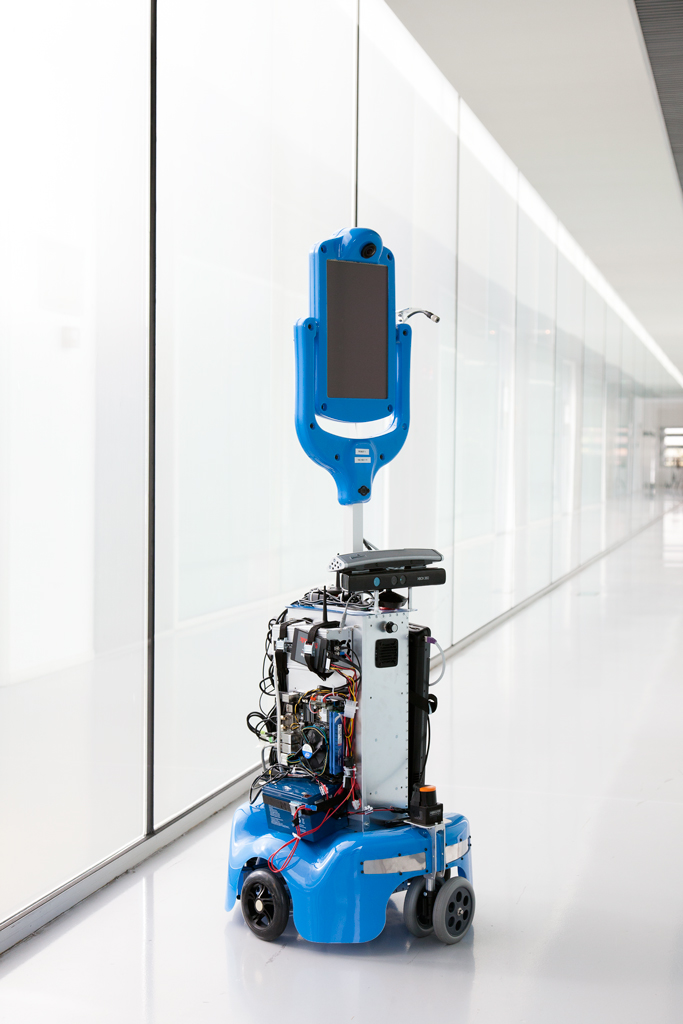
\includegraphics[scale = 0.13]{images/robot.jpg}

    \caption{}
       \label{fig:robot}
  \end{subfigure} 
  %\vspace{-3mm}
  \caption{(a) The data collected during a frame $(t)$ during our experiments.  (b) The TERESA robot. A telepresence robot with advanced sensing equipment was used to collect data in our experiments.}

    \vspace{-2mm}
  \label{fig:data_robot}
  \end{figure}

\section{Method}
In the previous sections we described the social tasks we will attempt to learn by demonstration. We have also described the data collection procedure that would allow us to do so. In this section we describe the learning architecture used to learn a mapping from robot observations to actions from this data. To derive this architecture we look closely into the data collected and the tasks at hand.
First we explain the type of learning we will perform namely, behavioral cloning, and argue that neural networks are an appropriate means of executing this learning procedure. We then build our network piece by piece by looking at different aspects of the data such as possible input representations, temporal aspects and the output mappings. 

\subsection{Behavioral Cloning}
There are several ways perform LfD in robots that have been studied extensively in the literature. The simplest and most straightforward of these is what is usually called behavioral cloning (BC). In BC we tackle LfD from a supervised learning (SL) perspective by treating the (sequences of) observations as input states $s_t$ and actions $a_t$ as labels, to train a \emph{policy} $\pi(s_t,a_t)$ so that similar actions are performed in similar situations. In this view any supervised learning paradigm (regression, classification) and algorithm (decision trees [], gaussian processes [], neural networks []) can be used to learn this policy from the data. Other forms of LfD exist, namely Inverse Reinforcement Learning [] which attempts to extract a cost function from the demonstrations that is subsequently used to plan (or learn []) a policy. IRL has been shown to be more data efficient and more transferable across environments. It is however harder apply in practice. IRL is certainly an interesting direction for future work however in this paper we use behavioural cloning because it is simpler and we are in possetion of enough data to perform learning.

Our choice of algorithm for learning the mapping function in this case is a Neural Network for two reasons. The first of these is \emph{generality}. In these paper our aim is to learn two (and potentially more) behaviours using a single algortithm. NNs can learn the features that are important for prediction automatically and this in turn means there would be therefore no need to define problem-specific features for a task, such as for example a group detection module. The second reason to use NNs is \emph{modularity}. This means that we can use different computation modules depending on our high level application. For example through recurrent neural networks we can easily deal with observations that vary (non linearly) over time in order to alleviate problems arising from noise in detections. Also in our input representation we have continuous as well as discrete variables, neural networks can deal with such representations easily. Finally, we are in this case outputing two values ($v,\omega$) and common supervised learning algorithms would treat each output independantly. This is ofcourse possible with methods other than neural networks, such as Gaussian Mixture Models (GMMs) or Hidden Markov Models (HMM), which would however require feature engineering to perform well.  

\subsection{Inputs and convolutional layers}
In the previous section we have seen that our observations at time t can be formulated as:

\begin{equation}
 	o_t = \{(\rho_1,\phi_1,1), (\rho_2,\phi_2,0),(\rho_3,\phi_3,0) ... (\rho_{K_t},\phi_{K_t},0)\}_t
\end{equation}
An important aspect of our observations is that the amount of people around the robot is dependent on time. This means that the size of our input vector would vary with time depending on the value of $K_t$. This is not very friendly for most learning algorithms that would expect a fixed input vector size. One way to alleviate this problem would be to fix $K$ to some number we consider reasonable. If the amount of people in the data is more than $K$ we would keep the $K$ closest. If the amount is smaller than $K$ we would simply fill the first $K$ positions of the vector and leave the last one with zeros. In this case however we are suggesting to the algorithm that there is a person on the robot since $\rho,\theta = (0,0)$. This could have adverse effects on learning, we could thus add another binary feature to our observation vector, to indicate wether the detection is a valid one. The new observation vector would thus look something like:

\begin{equation}
 	o_t = \{(\rho_1,\phi_1,1,1), (\rho_2,\phi_2,0,1),(\rho_3,\phi_3,0,1) ... (\rho_{K},\phi_{K},0,0)\}_t.
\end{equation}
Although perhaps inconvienient the above notation would give the learning algorithm all the information to learn a mapping. 

A more convienient representation however would be to imprint the observation on an image. This would involve fixing a maximum distance $x_{max},y_{max}$ from the robot and subsecuently painting all the people around the robot within that area on a ternary image. That is an image of three possible values, $0=$ no person is present, $1=$ a person is present, $2=$ a primary interaction target is present. We also denote the velocities of people as lines extending from the detections in the direction of the detected velocity and with a length that is representative of its magnitude. An example of such an image is shown in Figure ??. Another convienient aspect of this representation is that our image can contain further information such as for example the nearest non-human obstacles and the orientation of the people if this can be reliably detected. 

Although more convienient however this representation comes with a clear setback, which is that we are increasing the dimensionality of the problem. Usually when learning we seek to reduce the dimensionality of the problem through feature engineering, here we are in a sense doing the opposite. 

On the other hand the kind of images we are creating here are highly structured since we are only painting circles and lines. This means increase in dimensionality would no longer be problematic using methods that can easily capture and learn from structured images, such as convolutional neural networks []. 

Our analysis in the next section we go a step further to show that in practice this representation is not only more convienient but beneficial to learning.

IN ORDER TO MAKE THIS CLAIM. YOU NEED TO BE ABLE TO SHOW THAT THE CONVOLUTIONAL LAYERS LEARN A NON TRIVIAL FILTER BASIS, OTHERWISE WHAT YOU ARE SAYING IS BULLSHIT. WHY USE CONVOLUTIONAL LAYERS AND NOT SIMPLY A circle detector. I guess that without any figures your only reason would be that by combining these you might discover relationships between people. You really need to get the weights of those networks to see what they look like.  


\subsection{Dynamics and long short term memory}
Using a single observation as input to a convolutional neural network that outputs a control is unlikely to succesful for two main reasons.

\begin{itemize}
\item A single observation instance $o_t$ does not contain higher order information such a the acceleration of peole.
\item The people detection module is not perfect. False positives and negatives are common within the data, not having context information from previous observations will affect robustness of the controller.
\end{itemize}

Long-short term memory is a de-facto standard way of dealing with time depdendent output in neural networks. The LSTM is a type of Recurrent Neural Network (RNN) i.e., a neural network that can process time dependent inputs. In contrast with vanilla versions of RNNs however and LSTM is robust to unstable gradient phenomena often encountered during training of deep networks. In our architecture we use LSTMs to deal with the time dependent nature of the problem and achieve robustness in the face of uncertain detections.



\subsection{Outputs and Loss Functions}


\subsection{Continuous Learning Pipeline}
One major setback of behavioural cloning that has been studied in the literature, is that since most demonstrations are noisy examples of what the robot should do, the robot never learns how to get out of difficult situations when it finds itself in one, because it was never encountered in the data. For this reason we take a similar approach to the one encountered in []. First we collect some data using the robot, perform learning and deploy the learned policy on the robot. During execution we correct the robot whenever it makes a mistake, record the data from the intervention and then hand the control back to the robot.

% 	In this section, we propose Rapidly Exploring Learning Trees (RLT$^*$).  We first propose a generic extension to MMP that we call Approximate Maximum Margin Planning.  We then show how an implementation of this approach with an RRT$^*$ planner and a novel caching scheme yields RLT$^*$.

% 	% \subsection{Feature Sums and Sampled Based Planners}
% 	% 	Feature sums, $F(\zeta)$, can be seen as the  `fingerprints' of paths, and their definition is of crucial importance in the inverse problem. When planning on a fixed graph, like in the case of MDPs or A$^*$ search, it is easy to define the feature sums as the \emph{edge} costs on the graph. Furthermore if planning in continous domains we may consider integrals along the path. In RRT's however the tree that is being built has neither a fixed structure, nor an analytical form. Thus, the first step towards learning RRT$^*$ cost functions from demonstration is to come up with a reasonable approximation of $F(\zeta)$ for a path. This approximation must be consistent with the definition of the cost for a configuration pair. One such definition for cost is as follows.
% 	% 	\begin{equation}
% 	% 		c(s_i,s_j) = \frac{c(s_i)+c(s_j)}{2}d_{s_i,s_j}
% 	% 	\end{equation}
% 	% 	Where $c(s_i)$ is a cost function defined over a single configuration and $d_{s_i,s_j}$ is a measure of distance between the two configurations. For example if we consider configurations to be points in Eucledian space then $d_{s_i,s_j}$ can be the eucledian distance. Noting that the costs and features are related by \eqref{eq:inner_prod} for a single feature $f_k$ we have,

% 	% 	\begin{equation}
% 	% 		f_k(s_i,s_j) = \frac{f(s_i)+f(s_j)}{2}d_{s_i,s_j}
% 	% 	\end{equation}
% 	% 	Following this definition feature sum calculation along a candidate path is trivial,
% 	% 	\begin{equation}
% 	% 		F(\zeta) = \sum_{i=0}^{\zeta_l-1} \frac{\mathbf{f}(s_i)+\mathbf{f}(s_{i+1})}{2}d_{s_i,s_{i+1}}
% 	% 	\end{equation}

% 	\subsection{Approximate Maximum Margin Planning \label{subsec:ammp}}

% Section \ref{subsec:inverse_problem} shows how the multiple constraints of \eqref{eq:const1} can be reduced to the single constraint of \eqref{eq:const} for each demonstration. However, this reduction requires an optimal planner to perform the minimisation in \eqref{eq:const1}, which is impractical in many robot applications. Suppose instead that, as in RRT$^*$, we have a mechanism for sampling different paths from $Z_{o,g}$ along with their respective costs and that, for a given finite time budget $T$, this path sampler samples a subset $\tilde{Z}_{o,g} \subset Z_{o,g}$,  Then, we can modify \eqref{eq:const} to demand that our cost function satisfies,
% \begin{equation}
% 	C(\zeta^i_{o_i,g_i}) \leq \min_{\zeta_{o_i,g_i} \in \tilde{Z}_{o_i,g_i}} C(\zeta) \quad \forall i. \label{eq:const_rrt}
% \end{equation}
% 	As $T$ increases, lower cost paths are sampled, making this inequality harder to satisfy. Assuming $\tilde{Z}_{o_i,g_i}$ is constant, we can rewrite \eqref{eq:unconstrained} as:

% 	\begin{equation} \frac{1}{2}||\mathbf{w}||^2 + \frac{\lambda}{D} \sum_i \big( C(\zeta^i_{o_i,g_i}) - \min_{\zeta \in \tilde{Z}_{o_i,g_i}}\big(C(\zeta) + L_i(\zeta)\big) \big). \label{eq:unconstrained_rrt}
% 	\end{equation}
% This gives rise to an approach we call Approximate Maximum Margin Planning (AMMP). It is similar  to MMP with the crucial difference that the planning step is executed by a sample-based planner and not a deterministic one, like A$^*$. An important consequence is that $\tilde{Z}_{o_i,g_i}$ changes every time we invoke the sample-based planner. Thus, AMMP can be thought of as sampling the \emph{constraints} that we want our cost function to satisfy. The main advantage of AMMP is that it is not bound by the restrictive assumptions of  A$^*$, such as a discrete state-action space and no motion constraints. 

% However, an ineffective sampler could yield poor gradient estimates and thus poor solutions. In fact, Ratliff et al.\ \cite{ratliff2009chomp} argue that, for this reason, sample-based planners like RRT are not suited to learning cost functions from demonstration, as the paths sampled by RRT are heavily biased during the sampling process and thus highly suboptimal. However, asymptotically optimal sample-based planners like RRT$^*$ are better able to plan low-cost paths \cite{karaman2011sampling} and thus well suited for use within AMMP.

% \subsection{Rapidly Exploring Learning Trees \label{subsec:cached}}

% As suggested above, a simple way implement AMMP is to use RRT$^*$ as the sample-based planner.  RRT$^*$ can sample low-cost paths, allowing AMMP to learn a good cost function. Furthermore, RRT$^*$ can cope with large and continuous state-action spaces with motion constraints. However, the result is a computationally expensive algorithm that calls the planner $I\times|D|$ times over $I$ iterations, given a dataset of size $|D|$. Furthermore, sampling a separate set of points at every iteration could produce noisy gradients that negatively affect convergence. In this section, we propose Rapidly Exploring Learning Trees (RLT$^*$), which implements AMMP with an RRT$^*$ planner using a novel caching scheme to ensure both computational efficiency and more consistent gradients.

% A key observation is that, in RRT$^*$, only the rewiring step depends on the cost function.  The sampling step is independent of it and, especially when motion constraints are present, contains the most computationally expensive operations. These are: 1) fitting and querying a data structure to find the nearest neighbour and the radius neighbours to a newly sampled point, 2) applying the steer function to all neighbours to and from the newly sampled point, and 3) checking for obstacles in these paths. By contrast,  the only potentially expensive operation in the rewiring step is querying the cost of an edge. 

% Therefore, a key idea behind RLT$^*$ is to perform the sampling step just once for each data point and cache it for reuse throughout learning. Then, at each iteration, only the rewiring step needs to be repeated as the cost function changes.

% Algorithm \ref{alg:rrt_cache} describes the caching step, which takes as input $p$, the number of points to randomly sample from free space; $s_{init}$, the initial point; and $\eta$, the steer step size. For each randomly sampled point $s_{rand}$, we find the nearest neighbour, $s_{nearest}$, from the set of points in the vertex set $V$. We then create a new configuration point $s_{new}$ by steering from $s_{nearest}$ to $s_{rand}$. Next, we query the radius neighbours, $S_{near}$, of $s_{new}$ at a radius determined by  $\min\{\gamma_{RRT^*}(\frac{\log(|V|)}{|V|})^{\frac{1}{d}},\eta\}$. Here, $d$ is the dimensionality of $S$, and $\gamma_{RRT^*}$ is a constant based on the volume of free space (see \cite{karaman2011sampling}).  Next, we determine which points in $S_{near}$ can safely reach $s_{new}$ through the chosen \texttt{Steer} function (lines 13-17). These forward paths are stored in $Paths_{fwd}$. We then perform the same procedure but this time checking the paths from $s_{new}$ to $S_{near}$ and store them in the set $Paths_{bwd}$ (lines 18-22). This algorithm turns the sampling process of RRT$^*$  into a preprocessing step. Consequently, the expensive \texttt{Nearest}, \texttt{Near}, \texttt{Steer} and \texttt{Safe} procedures only need to be repeated $|D|$ times instead of $I\times|D|$ times.


% 	\begin{algorithm}
% 	 \algsetup{linenosize=\tiny}
%  	\scriptsize
% 	\caption{\small \texttt{cacheRRT}($n$,$s_{init}$,$\eta$)}
% 	\label{alg:rrt_cache}
% 	\begin{algorithmic}[1]
% 	\STATE $P \gets \emptyset$ \hfill \COMMENT{Initialise the point cache}
% 	\STATE $V \gets {s_{init}}$
% 	\FOR{$i=0 \dots n $}
% 	\STATE $s_{rand} \gets SampleFree_i$
% 	\STATE $s_{nearest} \gets \texttt{Nearest}(V,s_{rand})$
% 	\STATE $s_{new} \gets \texttt{Get}(s_{nearest},s_{rand})$
% 	\STATE $S_{near} \gets \texttt{Near}(V,{s_{new}},\min\{\gamma_{RRT^*}(\frac{\log(|V|)}{|V|})^{\frac{1}{d}},\eta\})$
% 	\STATE $Paths_{fwd} \gets \emptyset$
% 	\STATE $Paths_{bwd} \gets \emptyset$
% 	\STATE $S_{fwd} \gets \emptyset$
% 	\STATE $S_{bwd} \gets \emptyset$
% 	\FOR{$s_{near} \dots S_{near}$}
% 	\STATE $path_{fwd} = \texttt{Steer}(s_{near},s_{new})$
% 	\IF{$\texttt{Safe}(path_{fwd})$}
% 	\STATE $Paths_{fwd} \gets Paths_{fwd} \cup path_{fwd}$
% 	\STATE $S_{fwd} \gets S_{fwd} \cup s_{near}$
% 	\ENDIF
% 	\STATE $path_{bwd} = \texttt{Steer}(s_{new},s_{near})$
% 	\IF{$\texttt{Safe}(path_{bwd})$}
% 	\STATE $Paths_{bwd} \gets Paths_{bwd} \cup path_{bwd}$
% 	\STATE $S_{bwd} \gets S_{bwd} \cup s_{near}$
% 	\ENDIF
% 	\ENDFOR
% 	\STATE $V\gets V \cup s_{new}$
% 	\STATE $P \gets P \cup \{s_{nearest},s_{new},S_{fwd},S_{bwd},Paths_{fwd},Paths_{bwd}\}$
% 	\ENDFOR
% 	\RETURN $P$
% 	\end{algorithmic}

% 	\end{algorithm}


% The output of Algorithm \ref{alg:rrt_cache} is input to Algorithm \ref{alg:plan_cached}, which resembles the rewiring procedure in RRT$^*$ \cite{karaman2011sampling} and returns a low-cost path to the goal. However, unlike RRT$^*$ rewiring, the vertices of the tree and their neighbours at each iteration are already known and contained within the point cache. This speeds computation while keeping consistency between the planners used during learning and final execution. As learning proceeds and the cost function changes, so does the wiring of this tree; however, the points involved do not change. %Note that, despite caching, Algorithms \ref{alg:rrt_cache} and \ref{alg:plan_cached} are consistent with the planning procedure of the RRT$^*$. Consequently, there is no discrepancy between the planner used during learning and execution.

% Algorithm \ref{alg:ammp} describes Rapidly Exploring Learning Trees (RLT$^*$), which uses Algorithms \ref{alg:rrt_cache} and \ref{alg:plan_cached}. First, we initialise the weights, either randomly or using a cost function that simply favours shortest paths. Then, for each datapoint $\zeta_i$, we calculate feature sums and run \texttt{cacheRRT}. The main learning loop involves cycling through all data points and finding the best path under a loss-augmented cost function. The feature sums of this path are calculated and subsequently the difference with the demonstrated feature sums is computed. At the end of each iteration, an average gradient is calculated and the cost function is updated. At convergence, the learned weights are returned.

% In addition to saving computation time, the use of caching encourages consistency between the gradients computed in each iteration, as they are estimated from the same sampled points.  The effect on the gradients, which resembles that of momentum \cite{polyak1964some}, can improve performance, as our results in the next section show.

% 	\begin{algorithm}
% 	\algsetup{linenosize=\tiny}
%  	\scriptsize
% 	\caption{\texttt{planCachedRRT$^*$}($P$,$s_{init}$,$c()$)}
% 	 \label{alg:plan_cached}
% 	\begin{algorithmic}[1]
% 	\STATE $E \gets \emptyset$
% 	\STATE $V \gets {s_{init}}$
% 	\FOR{$i=0 \dots |P| $}
% 	\STATE $(s_{nearest},s_{new}) \gets P_i$
% 	\STATE $(S_{fwd},S_{bwd}) \gets P_i$
% 	\STATE $(Paths_{bwd},Paths_{fwd}) \gets P_i$
% 	\STATE $V\gets V \cup s_{new}$
% 	\STATE $s_{min}\gets s_{nearest}$
% 	\STATE $c_{min}\gets \texttt{Cost}(s_{nearest}) + c(path_{s_{nearest},s_{new}})$
% 	%\FOR{$s_{fwd} \in S_{fwd} $}
% 	\FOR{$j=0 \dots |S_{fwd}| $}
% 	\STATE $s_{fwd} = S^j_{fwd}$
% 	\STATE $path_{fwd} = Paths^j_{fwd}$  
% 	\STATE $C_{near} \gets \texttt{Cost}(s_{fwd}) + c(path_{fwd})$
% 	\IF { $C_{near}<c_{new}$}
% 	\STATE $s_{min} \gets s_{fwd}; c_{min}\gets c_{near}$
% 	\ENDIF
% 	\ENDFOR
% 	\STATE $E \gets E \cup \{(s_{min},s_{new})\} $
% 	%\FOR{$s_{bwd} \in S_{bwd} $}
% 	\FOR{$j=0 \dots |S_{bwd}| $}
% 	\STATE $s_{bwd} = S^j_{bwd}$
% 	\STATE $path_{bwd} = Paths^j_{bwd}$
% 	\STATE $C_{new} \gets \texttt{Cost}(s_{new}) + c(path_{bwd})$
% 	\IF {$C_{new}<\texttt{Cost}(s_{near})$}
% 	\STATE $s_{parent} \gets \texttt{Parent}(s_{bwd})$
% 	\STATE $E \gets E  \smallsetminus {(s_{parent},s_{bwd})} \cup {(s_{new},s_{bwd})} $
% 	\ENDIF
% 	\ENDFOR
% 	\ENDFOR
% 	\STATE $\zeta_{min} \gets \texttt{minCostPath}(V,E,c())$
% 	\RETURN $\zeta_{min}$
% 	\end{algorithmic}
% 	\end{algorithm}



% 	\begin{algorithm}
% 	 \algsetup{linenosize=\tiny}
%   	\scriptsize
% 	\caption{\texttt{RLT$^*$}($D,p,\eta,\lambda,\delta$)\label{alg:ammp}}
% 	\begin{algorithmic}[1]
% 	\STATE $\mathbf{w} \gets \texttt{initialiseWeights}$
% 	\STATE $\mathbf{\tilde{F}} \gets \emptyset$
% 	\STATE $R \gets \emptyset$
% 	\FOR{$\zeta^i \text{ in } D$}
% 	\STATE $\tilde{F}_{\zeta^i} \gets \texttt{FeatureSums}(\zeta^i)$
% 	\STATE $\mathbf{\tilde{F}} \gets \mathbf{\tilde{F}} \cup \tilde{F}_{\zeta^i}$
% 	\STATE $r_i \gets \texttt{cacheRRT}(p,s_{init}^{\zeta^i},\eta)$
% 	\STATE $R \gets R \cup r_i $
% 	\ENDFOR
% 	\REPEAT
% 	\STATE $\nabla_{\mathbf{w}}\gets 0$
% 	\FOR{$ \zeta^i \text{in } D $}
% 	\STATE $c() \gets \texttt{getCostmap}(\mathbf{w}) + L(\zeta^i)$ 
% 	\STATE $r_i \gets R\{i\}$ ;	$\tilde{F}_i \gets \mathbf{\tilde{F}}\{i\}$ 
% 	\STATE $\zeta \gets \texttt{planCachedRRT}^*(r_i,x^i_{init},c())$
% 	\STATE $F_i \gets \texttt{FeatureSums}(\zeta)$
% 	\STATE $\nabla_{\mathbf{w}} \gets \nabla_{\mathbf{w}} + \tilde{F}_i - F_i $
% 	\ENDFOR
% 	\STATE $\nabla_{\mathbf{w}} \gets \mathbf{w} + \frac{\lambda}{|D|}\nabla_{\mathbf{w}} $
% 	\STATE $\mathbf{w} \gets \mathbf{w} - \delta\nabla_{\mathbf{w}} $
% 	\UNTIL{convergence}
% 	\RETURN $\mathbf{w}$

% 	\end{algorithmic}
% 	\end{algorithm}

% 	% \STATE $\widetilde{\mu}^{\mathcal{D}} \gets \mathtt{empiricalFE}(\mathcal{D})$\hfill \COMMENT{using \eqref{eqn:empirical_fe}}
% 	% \STATE $\widetilde{\mu}^{\mathcal{F}} \gets \mathtt{empiricalFE}(\mathcal{F})$ 
% 	% \STATE $P_{\mathcal{D}}^{s_1} \gets \mathtt{initialStateDistribution}(\mathcal{D})$
% 	% \STATE $P_{\mathcal{F}}^{s_1} \gets \mathtt{initialStateDistribution}(\mathcal{F})$
% 	% \STATE $w^{\mathcal{F}}_k\gets 0\quad\forall k\in\{1,\ldots,K\}$
% 	% \REPEAT
% 	% \STATE $R(s,a) \gets (w^{\mathcal{D}}+w^{\mathcal{F}})^T\phi(s,a)\quad\forall s\in\mathcal{S},a\in\mathcal{A}$
% 	% \STATE $\pi \gets \mathtt{softPlan}(\mathcal{S},\mathcal{A},T,R)$\hfill\COMMENT{using \eqref{eq:soft_backup}}
% 	% \STATE $\mu^\pi|_{\mathcal{D}} = \mathtt{calculateFE}(\pi,T,P_{\mathcal{D}}^{s_1})$
% 	% \STATE $\mu^\pi|_{\mathcal{F}} = \mathtt{calculateFE}(\pi,T,P_{\mathcal{F}}^{s_1})$
% 	% \STATE $w^{\mathcal{D}} \leftarrow w^{\mathcal{D}} - \alpha (\mu^\pi|_{\mathcal{D}} - \widetilde{\mu}^{\mathcal{D}})$
% 	% \STATE $w^{\mathcal{F}} \leftarrow \frac{(\mu^\pi|_{\mathcal{F}} - \widetilde{\mu}^{\mathcal{F}})}{\lambda}$

% 	% \IF {$\lambda > \lambda_{min}$}
% 	% \STATE $\lambda \leftarrow \alpha_{\lambda}\lambda$
% 	% \ENDIF
% 	% \UNTIL{convergence}
% 	% \RETURN $R,\pi$


% For RRT$^*$, the dependance of $\tilde{Z}_{o_i,g_i}$ on the time budget T is hard to quantify since it depends on the size and nature of $S$ as well as the cost function we are using, which also changes with every iteration. For this reason, we resort to an experimental assessment of the ability of RRT$^*$ to sample the right constraints at every iteration of RLT$^*$ and hence effectively learn a cost function from demonstration.

% \section{Experiments}

% We evaluate RLT$^*$ by comparing it to MMP, implemented using an A$^*$ planner, and RLT$^*$-NC, an ablated version of RLT$^*$ that does not use caching.  We consider three experimental settings: 1) a simulated holonomic robot, 2) a simulated non-holonomic robot, and 3) a real telepresence robot.
	
% 	Our experiments take place in the context of socially intelligent navigation. IRL has been widely used in this setting \cite{henry2010learning,vasquez2014inverse,okallearning} because it is usually infeasible to hard-code the cost functions that a planner should use in complex social situations. Having the ability to quickly and effectively learn social navigation cost functions from demonstration would be a major asset for robots that operate in crowded environments such as airports \cite{triebel2015spencer}, museums \cite{thrun1999minerva} and care centres \cite{shiarlis2015teresa}.
	
% 	\subsection{Simulated Experiments}
% 	We first consider randomly generated social environments in simulation, such as the one shown in Figure \ref{fig:exp_setting}. Each arrow in the figure represents a person's position and orientation. The robot is given the task of navigating from one point in the room to another. While it is aware of the orientation and position of different people, it has no idea how to trade off reaching the target quickly with avoiding people and obstacles, i.e., the cost function is unknown. Instead, the robot is given a dataset of demonstrations $D$. Each demonstration $\zeta_i$ is a set of configurations $s = (x,y)$ representing positions of the robot in the configuration space and each demonstration takes place for a different random configuration of the social environment, i.e., the people are at different positions and orientations every time. The task is to use $D$ to extract a cost function that enables socially intelligent behaviour.

% 	\begin{figure}[tbh]
% %	\hspace{-5cm}
% 	\centering
%       \begin{subfigure}[b]{0.35\columnwidth}
%     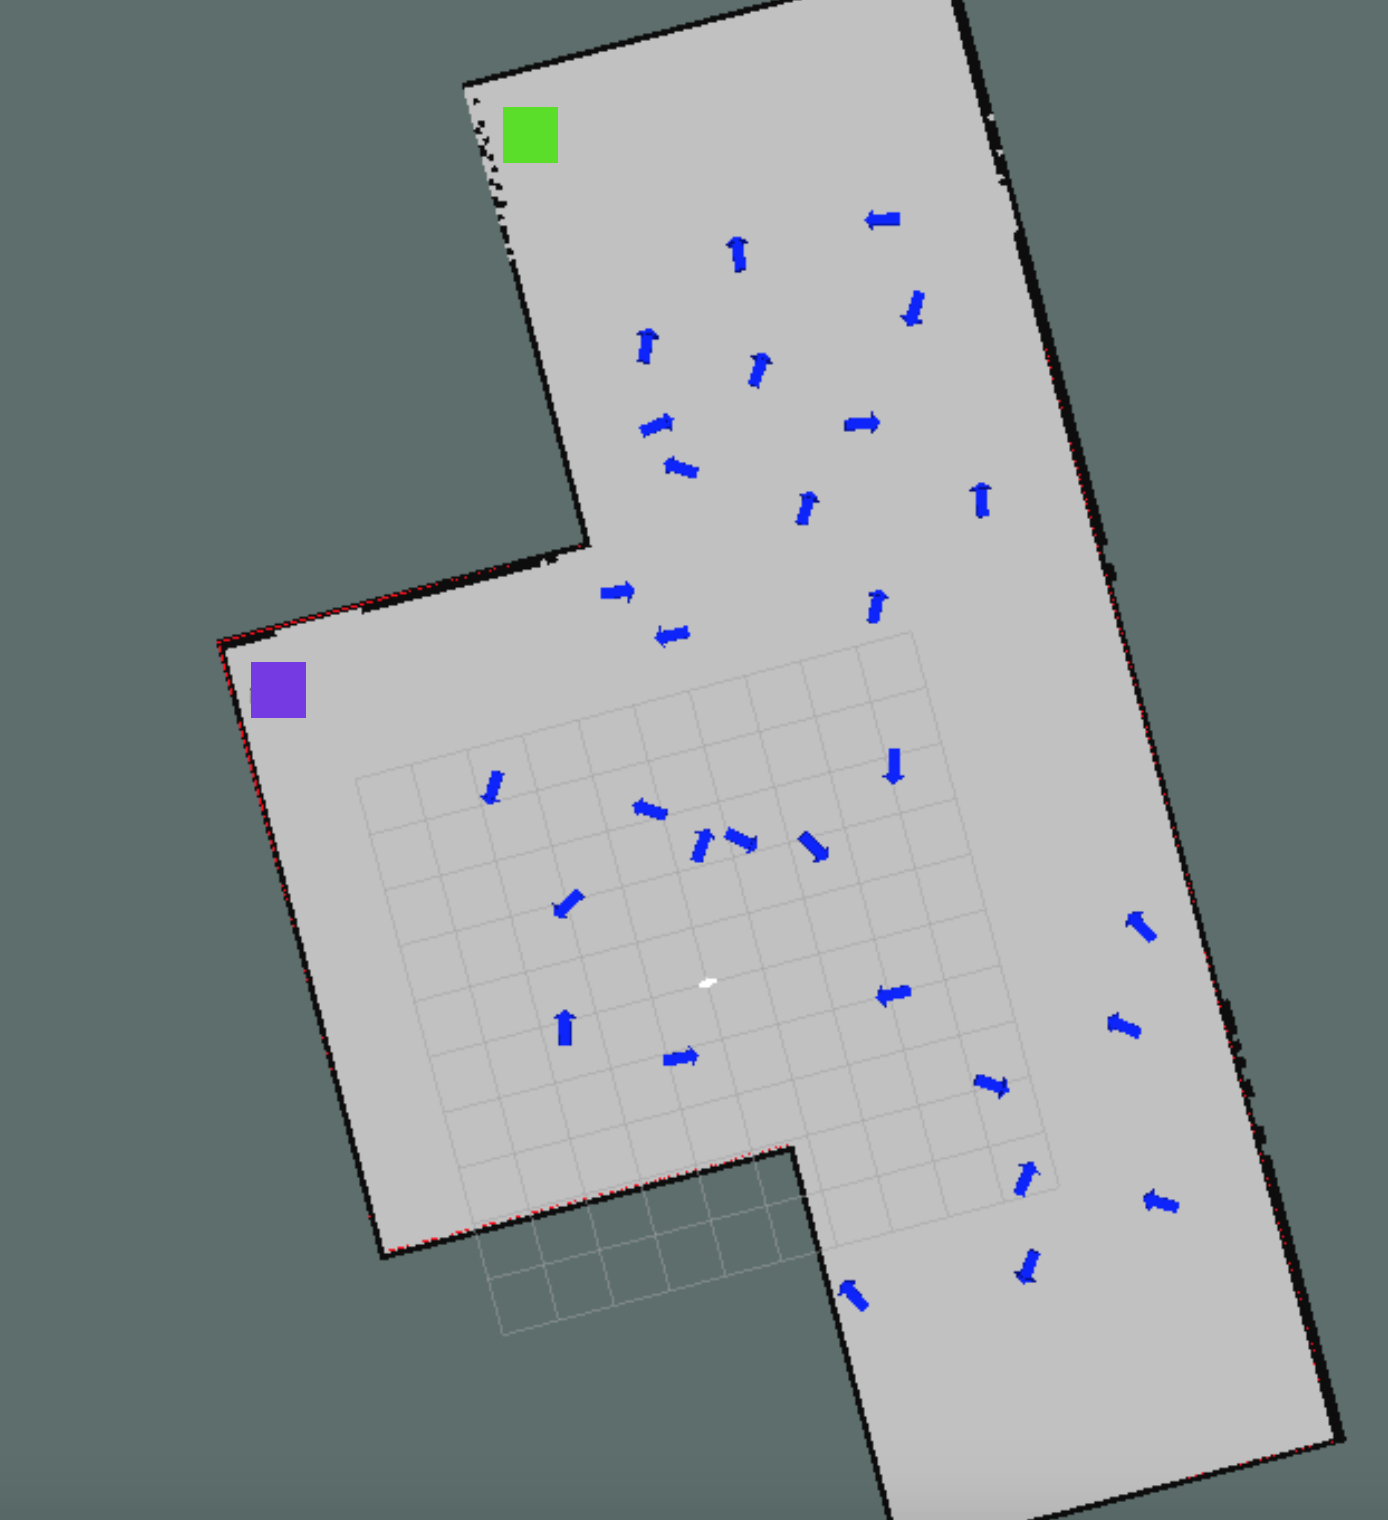
\includegraphics[scale = 0.15]{images/no_cf.png}
%     \caption{Example setting }
%     \label{fig:exp_setting}
%   \end{subfigure}
%   \hspace{10mm}
%   \begin{subfigure}[b]{0.35\columnwidth}
%   \hspace{4mm}
%     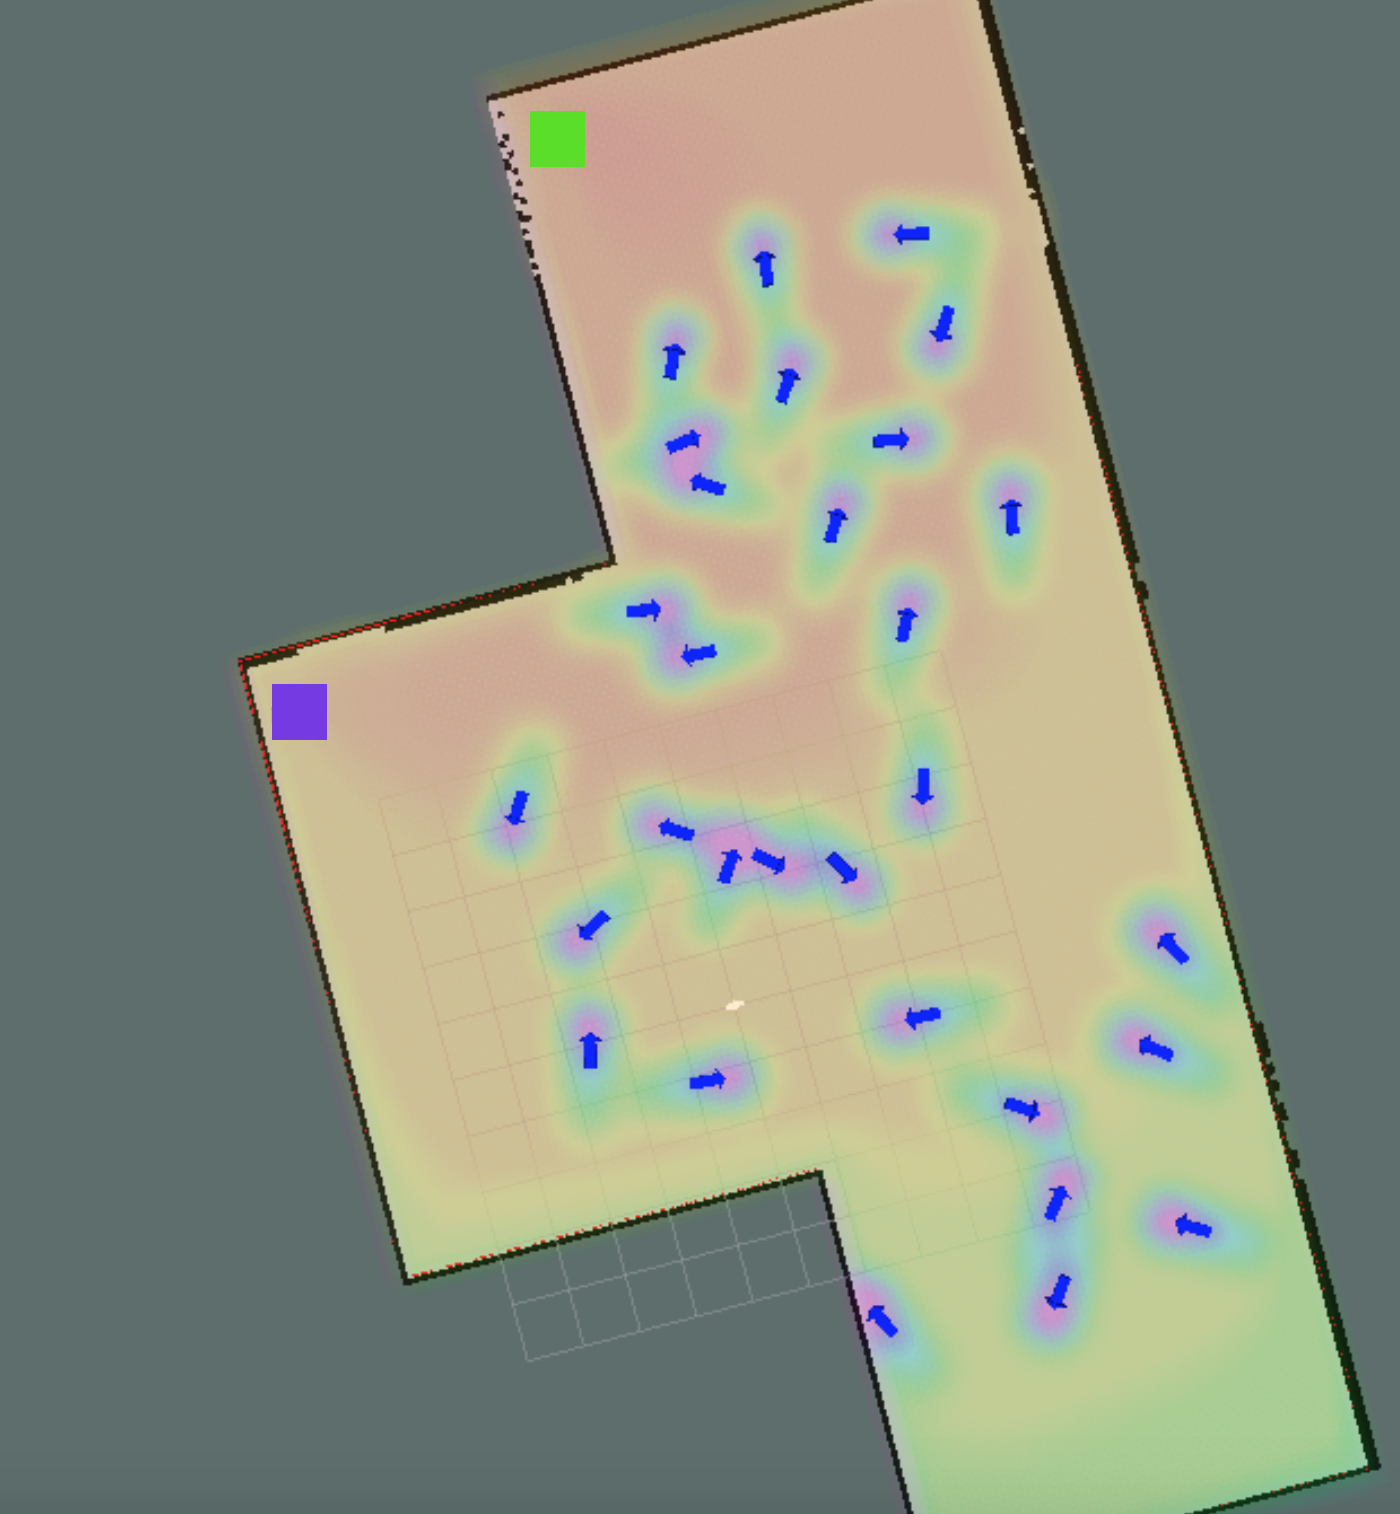
\includegraphics[scale = 0.15]{images/cf.png}
%     \caption{Cost function}
%     \label{fig:cost_f}
%   \end{subfigure} 

%   %\vspace{-3mm}
%   \caption{(a) A randomised instance of the social navigation task. Arrows denote the position and orientation of people in the scene. The robot is represented by the magenta box and the goal location is represented by the green box. (b) The corresponding cost function. Red denotes \emph{low} cost, while purple denotes \emph{high} cost.}

%     \vspace{-2mm}

%   %\vspace{-3mm}
%   \label{fig:setting}
%   \end{figure}

% 	The features we use can be divided into three categories. The first category encodes proxemics to the people present in the scene, i.e., the social features. Within this category we consider two variations, for reasons explained in the following section.
% 	\begin{itemize}
% 		\item {\bf Social feature set 1 (S1)}: Three isotropic Gaussian functions with different means, centred in front, behind, and on the person.
% 		\item {\bf Social feature set 2 (S2)}: Three field-of-view features. The features have a value of 1 if the robot is within a certain distance and angle from the person.
% 	\end{itemize}
% 	  The second category of features encodes the distance from the target location using linear, exponential, and logarithmic functions. The third category encodes the obstacle cost using a stable function of the reciprocal of the distance from the nearest obstacle. Figure \ref{fig:cost_f} shows an example cost function over the whole configuration space for the configuration in Figure \ref{fig:exp_setting}. We use different functions for human and target proximity, to allow for more degrees of freedom when modelling the underlying cost function. Sufficient regularisation ensures that that the model does not overfit.



% % 	\begin{figure}[tbh]
% % %	\hspace{-5cm}
% % 	\centering
% %       \begin{subfigure}[b]{0.42\columnwidth}
% %     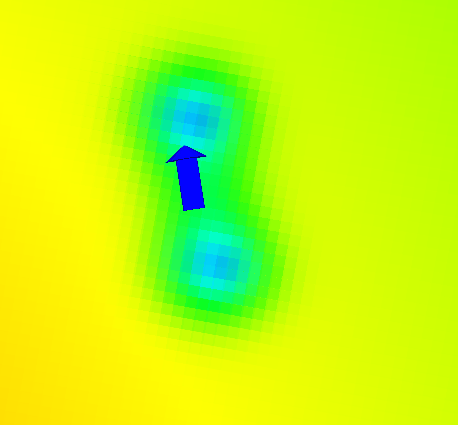
\includegraphics[scale=0.2]{images/person_feat2.png}
% %     \caption{Social feature set S1.}
% %     \label{fig:S1}
% %   \end{subfigure}
% %   \hspace{10mm}
% %   \begin{subfigure}[b]{0.42\columnwidth}
% %   \hspace{4mm}
% %     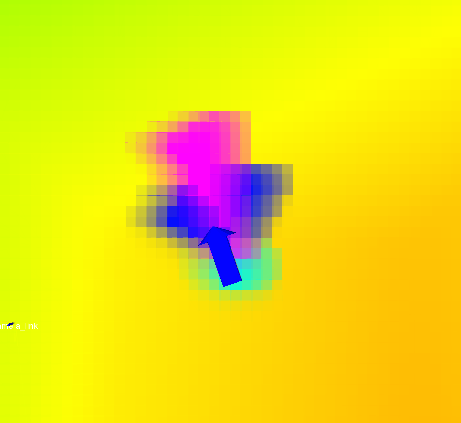
\includegraphics[scale=0.2]{images/person_feat1.png}
% %     \caption{Social feature set S2}
% %     \label{fig:S2}
% %   \end{subfigure} 
% %   %\vspace{-3mm}
% %   \caption{Cost functions resulting from linear combinations of the social featuresets. Figure \ref{fig:S1} demonstrates featureset 1. It consists of three isotropic Gaussian functions centered in front in the center and behind the person. Figure \ref{fig:S2} shows the field-of-view features of featureset S2. \sw{I have no idea what these plots are showing.} \ks{Now?}}
% %     \vspace{-2mm}
% %   %\vspace{-3mm}
% %   \label{fig:setting}
% %   \end{figure}


% 	\subsubsection{Evaluation}

% 	To evaluate our algorithms, we generate a dataset $D$ by planning near-optimal paths from initial configurations $s_o$ to goal configurations $s_g$ under a ground-truth cost function $c_{gt}()$ derived from ground-truth weights $\mathbf{w}_{gt}$ and features $\mathbf{F}_{gt}$. A fully optimal path can only be derived asymptotically in terms of either time  for RRT$^*$, or resolution for A$^*$. In practice, however, we found that planning for 100 seconds using  RRT$^*$  achieves a path that is nearly optimal; running longer leads to negligible changes in path cost. 
% 	The resulting ground truth dataset enables a quantatitive empirical evaluation, which is otherwise problematic in IRL \cite{vasquez2014inverse,shiarlis2016inverse}. For each path $\zeta$ generated by the learning algorithm, we know its cost under the ground-truth cost function and features is simply  $\mathbf{w}_{gt}^T\mathbf{F}_{gt}(\zeta)$. Furthermore, we can compute the \emph{cost difference} between the learned path and the demonstrated path with respect to ground truth:
% 	\begin{equation}
% 		Q(\zeta,\zeta_i,\mathbf{w}_{gt}) = \mathbf{w}_{gt}^T(\mathbf{F}_{gt}(\zeta)-\mathbf{F}_{gt}(\zeta_i)), \label{eq:obj_eval}
% 	\end{equation}
% which is our primary performance metric.  Note that, if the demonstration path $\zeta_i$ is optimal under $\mathbf{w}_{gt}$, then $Q(\zeta,\zeta_i,\mathbf{w}_{gt}) \geq 0$. For our holonomic simulated experiments, we consider two learning scenarios.
% \begin{enumerate}
% 	\item \textbf{Unknown weights}: only $\mathbf{w}_{gt}$ is unknown. The demonstrations and the learning algorithm share social feature set S1.
% 	\item \textbf{Unknown weights and features}: $\mathbf{w}_{gt}$ and $\mathbf{F}_{gt}$  are unknown. S2 is used to generate the demonstrations and S1 is used for learning.
% \end{enumerate}

% The first scenario evaluates each algorithm's ability to learn good cost functions when provided only with limited demonstrations of the task. The second scenario introduces a feature discrepancy to better simulate real-world settings, since it is unlikely that the features we define will exactly match those implicitly used by the human demonstrator.
% % In both cases the ground-truth weights $\mathbf{w}_{gt}$ were chosen to induce a cost function that penalises passing in front of people. In addition, small weights were added to the person related features, as well as linear and exponential penalisation of the distance from the goal, so that the cost functions would not be too trivial. 

% We also document the total learning time for K iterations for the algorithms under comparison.  All algorithms were implemented in Python, share similar functions, and were not optimised for speed apart from the caching scheme in RLT$^*$. Finally, we perform a qualitative evaluation by visually comparing the learned cost functions for each algorithm and the paths they generate against ground truth.

% 	\subsubsection{Holonomic Robot Results}

% 	Our dataset $D$ consists of 20 trajectories from random social social situations. We split $D$ into $D_{train}$ and $D_{test}$, each with 10 trajectories. After training on $D_{train}$, the cost difference of a cost function is evaluated on $D_{test}$ using \eqref{eq:obj_eval}. The process is repeated 7 times for the same dataset but with different random compositions of $D_{train}$ and $D_{test}$.  All learning algorithms are initialised using the same cost function that only favours shortest paths.
	
% 	As mentioned earlier, planning time and grid resolution affect the performance of RRT$^*$ and $A^*$, respectively. To make a fair comparison, we vary these two quantities for each algorithm and plot cost difference against learning time at each setting.  We can then identify which algorithms at which settings comprise the Pareto front, i.e., are undominated with respect to cost difference and learning time.
	
% 	 Figures \ref{fig:res_sim1} and \ref{fig:res_sim2} show the results for the two scenarios described earlier. MMP\_X (green) refers to MMP with X meters of grid resolution while  RLT\_X (red) and RLT$^*$-NC\_X (blue) refer to RLT and RLT without caching, respectively, with X seconds of planning. The shading represents an interpolation of the performance between settings for each method. In this way an area of single colour illustrates hypothesized domination of that method over another, given the same amount of time. Since lower is better for both cost difference and learning time, the closer a point is to the bottom left corner, the better.

% 	\begin{figure}[tbh]
% 	\centering
% 	\captionsetup[subfigure]{justification=centering}
% 	\hspace{-1cm}
%       \begin{subfigure}[b]{0.41\columnwidth}
%     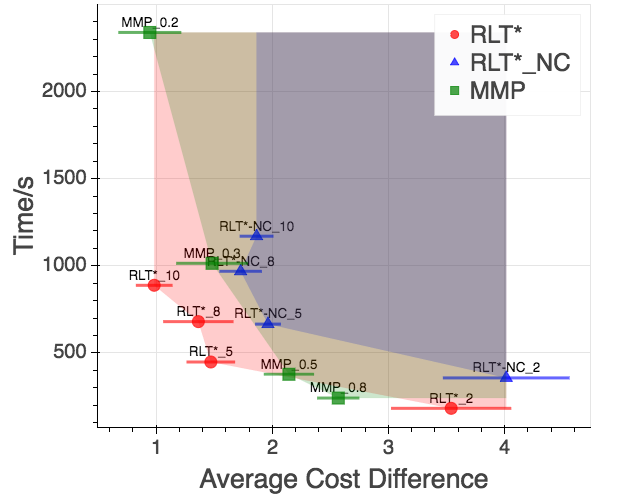
\includegraphics[scale=0.21]{images/pf_same.png}
%     \caption{Unknown weights scenario.}
%     \label{fig:res_sim1}
%   \end{subfigure}
%      	\hspace{10mm}
%   \begin{subfigure}[b]{0.41\columnwidth}

%     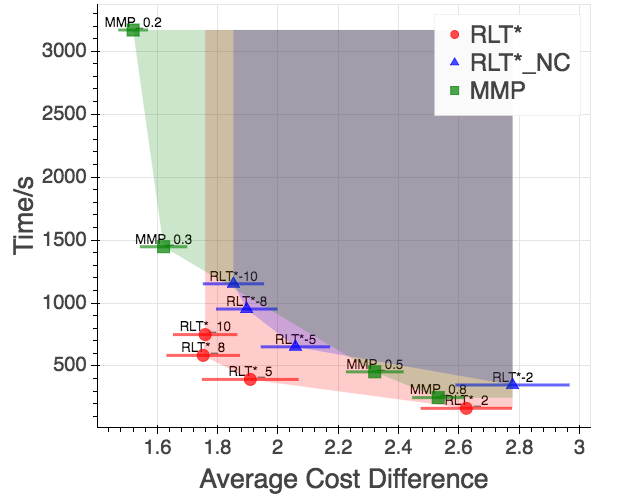
\includegraphics[scale=0.21]{images/pf_different.png}
%     \caption{Unknown weights and features scenario.}
%     \label{fig:res_sim2}
%   \end{subfigure} 
%     \caption{Learning time vs.\ cost difference on the holonomic robot for MMP (green), RLT$^*$-NC (blue), and RLT (red) at different planning fidelities. On both axes \emph{lower is better}.}
%     \vspace{-2mm}
%   %\vspace{-3mm}
%   \label{fig:results_sim}
%   \end{figure}

%  RLT$^*$ (red) comprises a large majority of the Pareto front, demonstrating good performance and generalisation in reasonable time.  However, the performance of RLT$^*$ and RLT$^*$-NC significantly degrades at very low planning times (2 seconds) because AMMP cannot sample good enough paths to compute a useful gradient.
 
%  Note that caching not only speeds learning in RLT$^*$, it also modestly reduces cost differences. This suggests that the caching scheme introduces extra robustness and generalisation capabilities within the algorithm.  As mentioned in Section \ref{subsec:cached}, we hypothesise that the caching scheme improves learning by making the gradients smoother and more consistent, as with momentum. To confirm this, we plot the inner product between successive gradients during learning in Figure \ref{fig:in_prod_grad}. The plot confirms that subsequent gradients in RLT$^*$ are more similar.
 
%  Finally, note that MMP's learning time scales exponentially with the size of the grid. This, however, is not solely due to the graph getting larger but also because A$^*$ search scales poorly with the complexity of the cost function itself. Since it relies on an admissible heuristic that for complex cost functions is no longer tight, A$^*$ must expand many more states.  RLT$^*$ is less susceptible to such problems.

%  	\begin{figure}[tbh]
% %	\hspace{-5cm}
% 	\centering
%     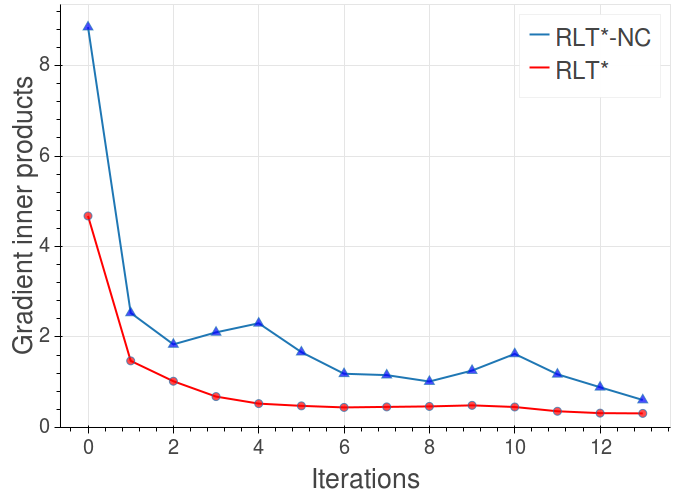
\includegraphics[scale=0.21]{images/momentum.png}
%     \caption{Inner product of succcessive gradients during learning. The smoother curve for RLT$^*$ suggests that fixing the sampled points during learning makes the gradients more consistent. }
%     \vspace{-2mm}
%   %\vspace{-3mm}
%   \label{fig:in_prod_grad}
%   \end{figure}


%   \subsubsection{Non-Holonomic Robot Results}
%   As mentioned earlier, a potential advantage of RLT$^*$ is that it can efficiently handle learning in the presence of motion constraints. In this section, we consider a robot planning in a three-dimensional space, $(x,y,\theta)$, representing the position and orientation of the robot. The robot's motion is further subject to the following motion constraints:
% %
%   \begin{align}
%   	&\dot{x} = v\times\cos(\theta),\\
%   	&\dot{y} = v\times\sin(\theta),\\
%   	&\dot{\theta} = \omega,
%   \end{align}
%   where $v,\omega$ are the linear and angular velocities respectively.
%   To meet these constraints, we use the POSQ $\texttt{Steer}$ function \cite{palmieri2014novel}.  Since this approach gives a local closed-loop policy between two vertices of the tree, it is  more robust to noise and uncertainty in the motion than an open loop trajectory. Furthermore, it has been shown to produce smooth paths between feasible configurations \cite{palmieri2014novel}. Evaluation is done in the same way as in the previous section, except that we compare RLT$^*$ only to RLT$^*$-NC and not MMP, as the latter cannot handle motion constraints.
% RLT$^*$-NC was given 100 seconds to plan, in which case about 3000 configurations were sampled, and RLT$^*$'s cache was set to this size. 

% Figure \ref{fig:results_kino} shows that RLT$^*$ is an order of magnitude faster than RLT$^*$-NC, while achieving a lower cost difference. The kinematic constraints contribute to this speedup since they make the \texttt{Steer} and \texttt{Safe} procedures, which are cached, more expensive. As in the holonomic case, RLT$^*$ resulted in smoother learning, confirming the results of Figure \ref{fig:in_prod_grad}. 

%   	\begin{figure}[tbh]
% 	\centering
% 	\captionsetup[subfigure]{justification=centering}
% 	\hspace{-1cm}
%       % \begin{subfigure}[b]{0.42\columnwidth}
%     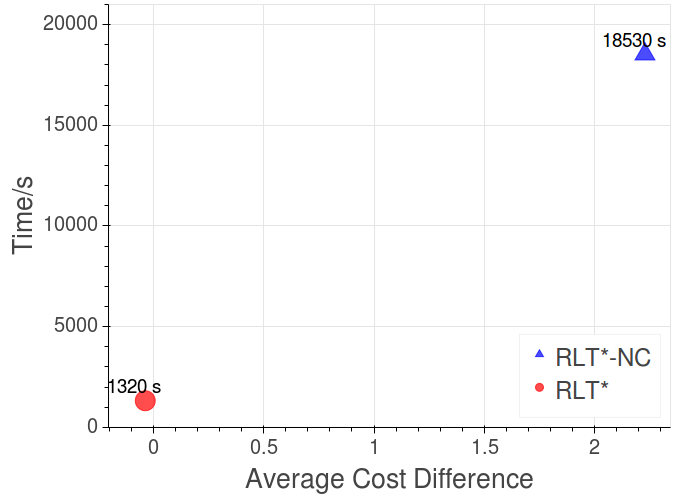
\includegraphics[scale=0.2]{images/pareto_front_kino.png}
%     % \caption{Learning time vs.\ cost difference.}
%     % \label{fig:res_kino1}
%   % \end{subfigure}
%      	% \hspace{10mm}
%   % \begin{subfigure}[b]{0.42\columnwidth}

%   %   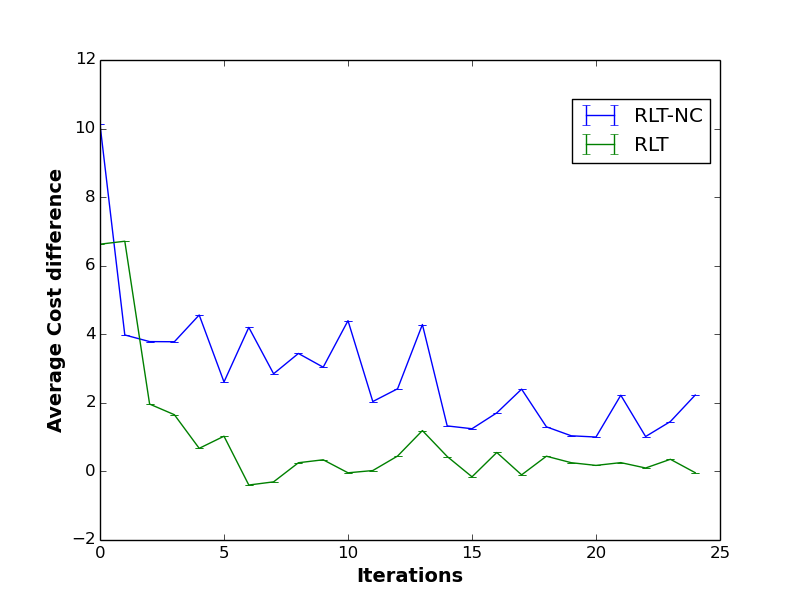
\includegraphics[scale=0.25]{images/cost_diff_val_kino.png}
%   %   \caption{Learning curve}
%   %   \label{fig:res_kino2}
%   % \end{subfigure} 
%     \caption{Non-holonomic robot results.}
%     \vspace{-2mm}
%   %\vspace{-3mm}
%   \label{fig:results_kino}
%   \end{figure}

% Figure \ref{fig:results_qual} shows an instance of the types of paths generated by our method when compared to ground truth. This specific example was drawn from the validation set and is thus not a case of overfitting.


% 	\begin{figure}[tbh]
% %	\hspace{-5cm}
% 	\centering
%     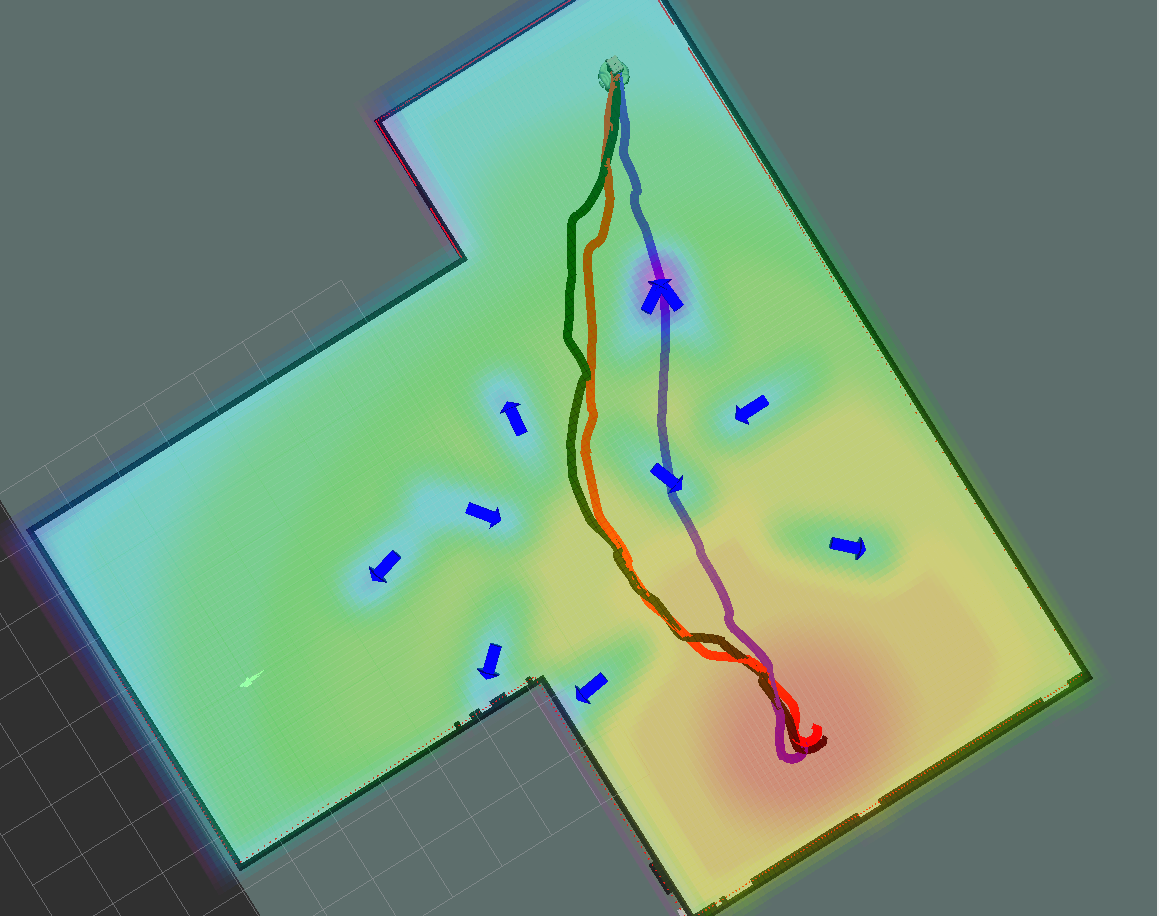
\includegraphics[scale=0.12]{images/kino_paths.png}
%     \caption{Qualitative evaluation of simulated results. The colour map denotes the learned cost function. Red denotes \emph(low) cost and green \emph{high} cost. The learned path (red) is quite similar to the demonstrated path (black) with a clear improvement over the path before learning (purple).}
%     \vspace{-2mm}
%   %\vspace{-3mm}
%   \label{fig:results_qual}
%   \end{figure}

% 	\subsection{Real Robot Experiments}
% 	In this section, we apply RLT$^*$ to real, human demonstrations using a telepresence robot, shown in Figure \ref{fig:robot}, in a social navigation scenario. Furthermore, we deploy the learned cost function on the actual robot.

%   	\begin{figure}[tbh]
% 	\centering
% 	\captionsetup[subfigure]{justification=centering}
% 	\hspace{-1cm}
%       % \begin{subfigure}[b]{0.42\columnwidth}
%     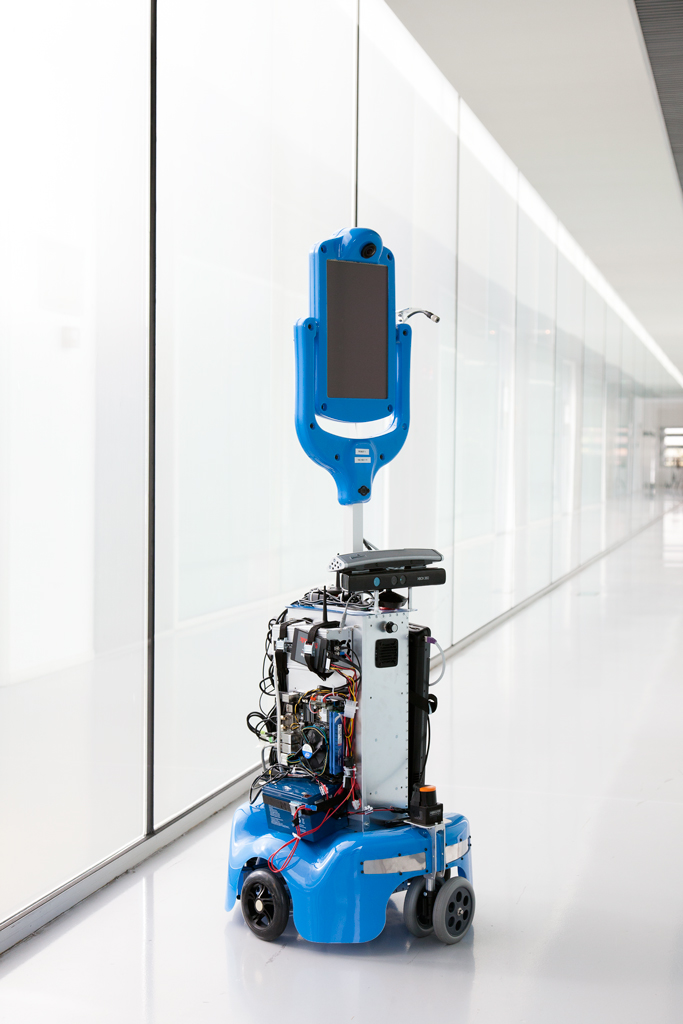
\includegraphics[scale=0.13]{images/robot.jpg}
%     % \caption{Learning time vs.\ cost difference.}
%     % \label{fig:res_kino1}
%   % \end{subfigure}
%      	% \hspace{10mm}
%   % \begin{subfigure}[b]{0.42\columnwidth}

%   %   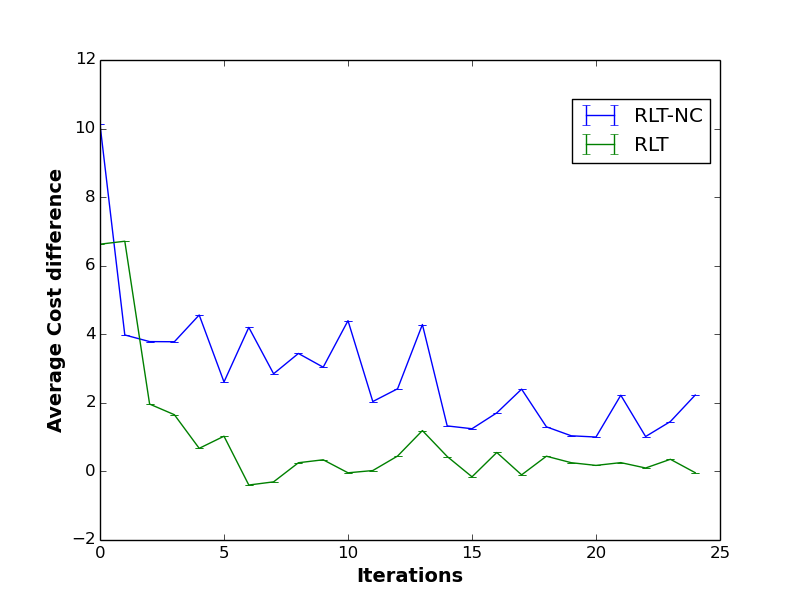
\includegraphics[scale=0.25]{images/cost_diff_val_kino.png}
%   %   \caption{Learning curve}
%   %   \label{fig:res_kino2}
%   % \end{subfigure} 
%     \caption{The telepresence robot used in our experiments.}
%     \vspace{-2mm}
%   %\vspace{-3mm}
%   \label{fig:robot}
%   \end{figure}

% 	The experiments take place in a simplified version of the social scenarios we have seen in the previous section. There are two people in the scene at different positions and orientations. A human demonstrator is asked to execute paths for different initial and final conditions across the room. The task is similar to the one used in \cite{okallearning} and the purpose is to find cost functions that account for potential relationships between people depending on their orientation with respect to each other. For example, if people are facing each other, they are  likely engaged in conversation or a similar activity (e.g., taking a photograph) that should not be interrupted. By contrast, if they are looking away from each other and there is enough distance between them then, it might be better to pass between them if doing so yields a shorter path.

% 	To collect data for learning and validation, we use an off-the-shelf telepresence system augmented with several sensors that allow localisation and perception \cite{shiarlis2015teresa}. We use an Optitrack motion capture system to accurately collect ground truth data of both people and robot positions. RLT$^*$ learns a cost function from this data using the social feature set S1 and the rest of the features described earlier.

% Since quantitative evaluation is difficult using real data, as no ground truth is available, we perform a qualitative evaluation instead. Figure \ref{fig:results_real} shows some representative cases that arose during learning. Figure \ref{fig:res_real1} shows a case where RLT$^*$ produced paths (red) that are quite similar to the demonstrated ones (black). Figure \ref{fig:res_real4} shows an instance instances where  the learned paths are reasonable even though they are not similar to the demonstrated paths.

% 			\begin{figure}[tbh]
% %	\hspace{-5cm}
% 	\centering
%       \begin{subfigure}[b]{0.42\columnwidth}
%     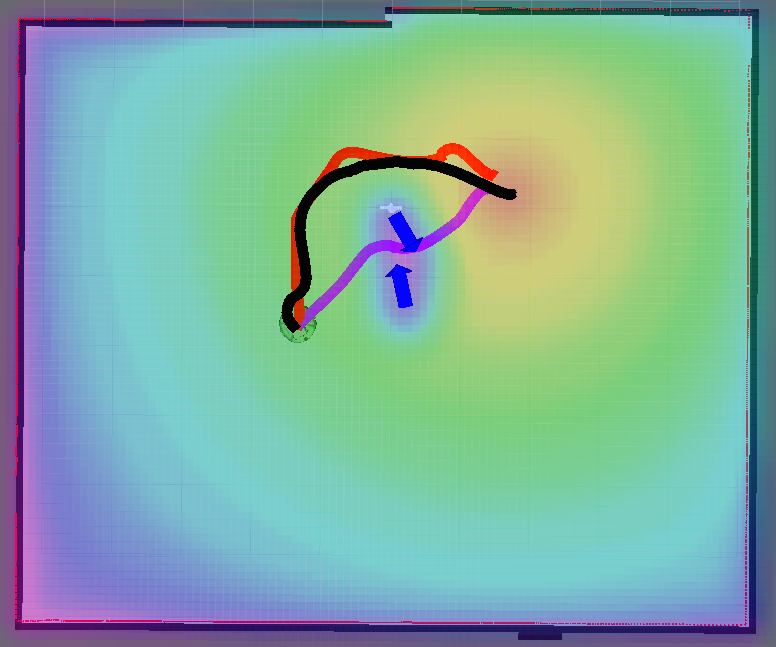
\includegraphics[scale=0.12]{images/real_good_new.png}
%     \caption{}
%     \label{fig:res_real1}
%   \end{subfigure}
%   \hspace{10mm}
%   \begin{subfigure}[b]{0.42\columnwidth}
%   \hspace{4mm}
%     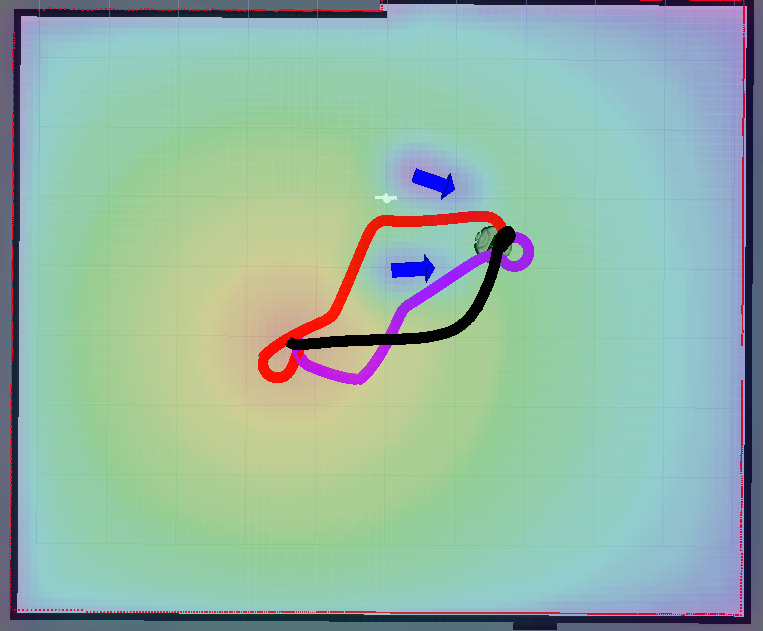
\includegraphics[scale=0.12]{images/real_reasonable_new.png}
%     \caption{}
%     \label{fig:res_real4}
%   \end{subfigure} 
%     \caption{Real demonstrated paths (black), learned paths (red), and shortest paths (purple). In (a), the learned path is similar to the demonstrated path; in (b) it is different but reasonable. The paths are laid over the learned cost function.}
%     \vspace{-2mm}
%   %\vspace{-3mm}
%   \label{fig:results_real}
%   \end{figure}


% 	Finally, we successfully deployed the learned cost function, also shown in Figure \ref{fig:results_real}, on a real telepresence robot. A video demonstrating this deployment can be found in the supplementary material. Even though our planner outputs a full policy in terms of angular and linear velocities, to follow the prescribed path we used an elastic bands local planner in order to deal with dynamic changes in the environment.%\ks{should I say this?} \jm{I think it's ok} 



% \vspace{-1mm}
% \section{Conclusion \& Future Work}
% In this paper, we proposed Rapidly Exploring Learning Trees (RLT$^*$), which learns the cost functions of Rapidly Exploring Random Trees (RRT) from demonstration, thereby making inverse learning methods applicable to more complex tasks. Our approach extends the Maximum Margin Planning to work with RRT$^*$ cost functions. Furthermore, it uses a caching scheme that greatly reduces the computational cost and improves performance. Our results in simulated social navigation scenarios show that RLT$^*$ achieves better performance at lower computational cost, even when there is a discrepancy between the features used for demonstration and learning. Furthermore, our results show that RLT$^*$ can handle more complex configuration spaces with motion constraints. Finally, we used RLT$^*$ to learn a cost function using data from real demonstrations on a telepresence robot and successfully deployed that cost function back on the robot.

% In future work, we hope to extend RLT$^*$ to model how features evolve over time, in order to, e.g., consider people's movement during planning.  For complex social path planning applications, periodic replanning has been shown to help \cite{henry2010learning,vasquez2014inverse}. Replanning in RRT$^*$ is also possible \cite{otte2015rrtx} and could potentially be incorporated into RLT$*$.

\bibliographystyle{IEEEtran}
\bibliography{references}



\end{document}
